\begin{frame}[t]{\ev{\tagA\,\tagB}\surf{COUNT ONCE}Overlapping trials add less than their count.}
\vspace{.15cm}
\begin{center}
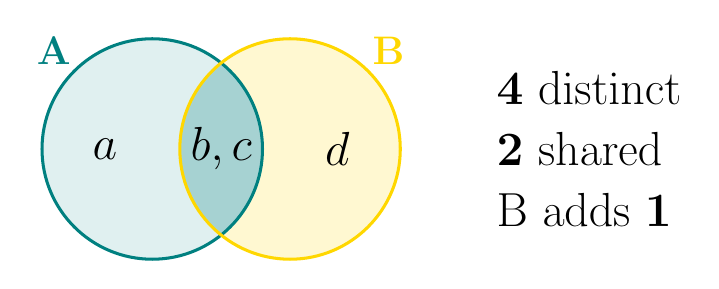
\begin{tikzpicture}[x=1cm,y=1cm]
% Two trials that return overlapping observation IDs.
\fill[Teal!12](0,0)circle(1.4);\fill[Gold!18](1.75,0)circle(1.4);
\begin{scope}\clip(0,0)circle(1.4);\fill[Teal!35](1.75,0)circle(1.4);\end{scope}
\draw[Teal,line width=1.1pt](0,0)circle(1.4);\draw[Gold,line width=1.1pt](1.75,0)circle(1.4);
\node[font=\fontsize{15}{18}\selectfont\bfseries,text=Teal] at (-1.25,1.25) {A};
\node[font=\fontsize{15}{18}\selectfont\bfseries,text=Gold] at (3.0,1.25) {B};
\node[font=\fontsize{18}{21}\selectfont] at (-.6,0) {$a$};
\node[font=\fontsize{18}{21}\selectfont] at (.875,0) {$b,c$};
\node[font=\fontsize{18}{21}\selectfont] at (2.35,0) {$d$};
\node[anchor=west,align=left,font=\fontsize{16}{22}\selectfont] at (4.25,0) {\textbf{4} distinct\\\textbf{2} shared\\B adds \textbf{1}};
\end{tikzpicture}
\end{center}
\vspace{.05cm}
{\centering\fontsize{12.5}{15}\selectfont\color{Muted}One road, many drives. One gene, six guides.\par}
\claim{A shared observation counts once.}
\vspace{.2cm}
{\centering\fontsize{12}{15}\selectfont\tagB\enspace Our reducer rejects duplicate observation IDs.\par}
\sources{Illustrative IDs. Callbacks: Roadbook drives, CRISPR guides. \href{https://github.com/zozo123/boltzmann-mapreduce}{Reference reducer}; \href{https://arxiv.org/html/2607.09689v4}{arXiv:2607.09689v4}.}

\qadetail{The set diagram counts exact illustrative observation IDs; circle areas do not represent entropy or Fisher information. Deduplicating declared IDs does not measure correlation between different items; distinct IDs do not authenticate observations or prove independence, and a copied receipt remains the same observation. The Roadbook and guide callbacks are analogies: matched drives of one road and six guides per gene are repeated looks at one target, not forks or measured correlations. The built Gaussian/Wald reference reducer adds natural-parameter summaries associatively under an independence/common-target model; a declared duplicate evidence ID raises; lineage is transported but not yet consumed. It does not abstain. Source: Eliaz, arXiv:2607.09689v4.}
\note{[0:50] The simplest thing trials share is an observation. Trial A returns a, b and c. Trial B returns b, c and d. That is four distinct observations, not six, so B adds only d. We have seen this before. The Roadbook counts a road once, however many drives cross it. Six guides aimed at one gene are six looks at one gene. Our reducer pools the results. Today, it rejects a duplicate observation ID. It also keeps each result's source history. But different observations can still share errors.}
\end{frame}
